\chapter{المرايا والانعكاس}\label{ch:g5:mirrors-reflection}

\omterm{def:g1:light-and-shadows:source}{الضوء}، كما برهنّا، لا ينثني حول الزوايا أبدًا --- ومع ذلك تطلّ
نسخة منك كل صباح من جدار الحمّام، وقد وعدنا في السنة الماضية
بحيلة تتيح الرؤية من وراء الزوايا رغم ذلك. والحيلة ليست أن يُثنى
الطريق بل أن \emph{يُطوى}. وكل شيء ينطوي عند سطح واحد عجيب:
\omterm{def:g5:mirrors-reflection:reflection}{المرآة}.

\section{الارتداد}

\begin{definition}[الانعكاس]\label{def:g5:mirrors-reflection:reflection}
حين يصطدم \omterm{def:g1:light-and-shadows:source}{الضوء} بسطح فيرتدّ بدل أن ينفذ منه أو يموت عنده نسمّي
ذلك \emph{انعكاسًا}\index{انعكاس}: فيقال إن \omterm{def:g1:light-and-shadows:source}{الضوء} انعكس.
و\emph{المرآة}\index{مرآة} سطح من الملاسة بحيث يعكس \omterm{def:g1:light-and-shadows:source}{الضوء}
انعكاسًا منظَّمًا تمامًا --- معدن مصقول خلف زجاج، أو ماء ساكن،
أو ملعقة لامعة.
\end{definition}

\begin{proposition}[قاعدة الارتداد]\label{prop:g5:mirrors-reflection:bounce}
يرتدّ شعاع \omterm{def:g1:light-and-shadows:source}{الضوء} عن \omterm{def:g5:mirrors-reflection:reflection}{المرآة} كما ترتدّ كرة مثالية عن جدار: فيغادر
بالميل نفسه الذي وصل به تمامًا، في الجهة الأخرى. عموديًّا داخلًا
--- عموديًّا راجعًا. ومائلًا داخلًا --- مائلًا خارجًا بالميل
الموافق. والزاويتان، زاوية الوصول وزاوية المغادرة، متساويتان
دائمًا.
\end{proposition}

\begin{omfigure}
\begin{tikzpicture}[scale=0.85]
  \draw[very thick] (0.5,0) -- (10.5,0);
  \foreach \x in {1.0,1.75,...,10.0} {
    \draw[thin] (\x,0) -- (\x-0.3,-0.3);
  }
  \draw[-Stealth, very thick, omThm] (2.0,3.0) -- (5.5,0.05);
  \draw[-Stealth, very thick, omThm] (5.5,0.05) -- (9.0,3.0);
  \draw[dashed] (5.5,0) -- (5.5,3.2);
  \draw[omExo, thick] (4.42,0.95) arc (140:90:1.45);
  \draw[omExo, thick] (6.58,0.95) arc (40:90:1.45);
  \node[font=\small] at (4.7,1.75) {وارد};
  \node[font=\small] at (6.35,1.75) {منعكس};
  \node[below, font=\small] at (5.5,-0.45)
    {ميلان متساويان على جانبَي الخطّ المتقطّع القائم};
\end{tikzpicture}

{\small قاعدة الارتداد: الشعاع المغادر يعكس الشعاع الوارد ---
زاويتان متساويتان على جانبَي العمود.}
\end{omfigure}

\begin{example}[تصويب الارتداد]\label{ex:g5:mirrors-reflection:aiming}
ولأن الارتداد بهذا الانتظام يمكن \emph{تصويبه}: فبمرآة صغيرة في
\omterm{def:g1:light-and-shadows:source}{ضوء} الشمس تستطيع أن تلقي بقعة \omterm{def:g1:light-and-shadows:source}{ضوء} على أيّ جدار تختاره --- أمِل
\omterm{def:g5:mirrors-reflection:reflection}{المرآة} تطعك البقعة. ويستعمل البحّارة والمتنزّهون في الشدّة هذا
بعينه: \omterm{def:g5:mirrors-reflection:reflection}{فمرآة} تومض مصوَّبة نحو سفينة بعيدة أو مروحية إشارة تُرى
من كيلومترات كثيرة، تشغّلها الشمس وحدها.
\end{example}

\begin{example}[لماذا ليست الجدران مرايا]\label{ex:g5:mirrors-reflection:walls}
الجدار الأبيض يعكس ضوءًا كثيرًا --- ولولا ذلك لكانت الغرفة
كئيبة --- فلماذا لا يُظهر صورة؟ عن قرب يكون سطحه مشهدًا من نتوءات
دقيقة: فيطيع كل شعاع وارد قاعدة الارتداد على ميله الصغير الخاص،
فيتبدّد جيش الأشعّة المنظَّم في كل الجهات. أما صقل \omterm{def:g5:mirrors-reflection:reflection}{المرآة} فيبقي
الميول مستوية، فيبقى الجيش منتظمًا، وتنجو الصورة من الارتداد.
فالنظام، لا اللمعان وحده، هو صانع الصورة.
\end{example}

\begin{omfigure}
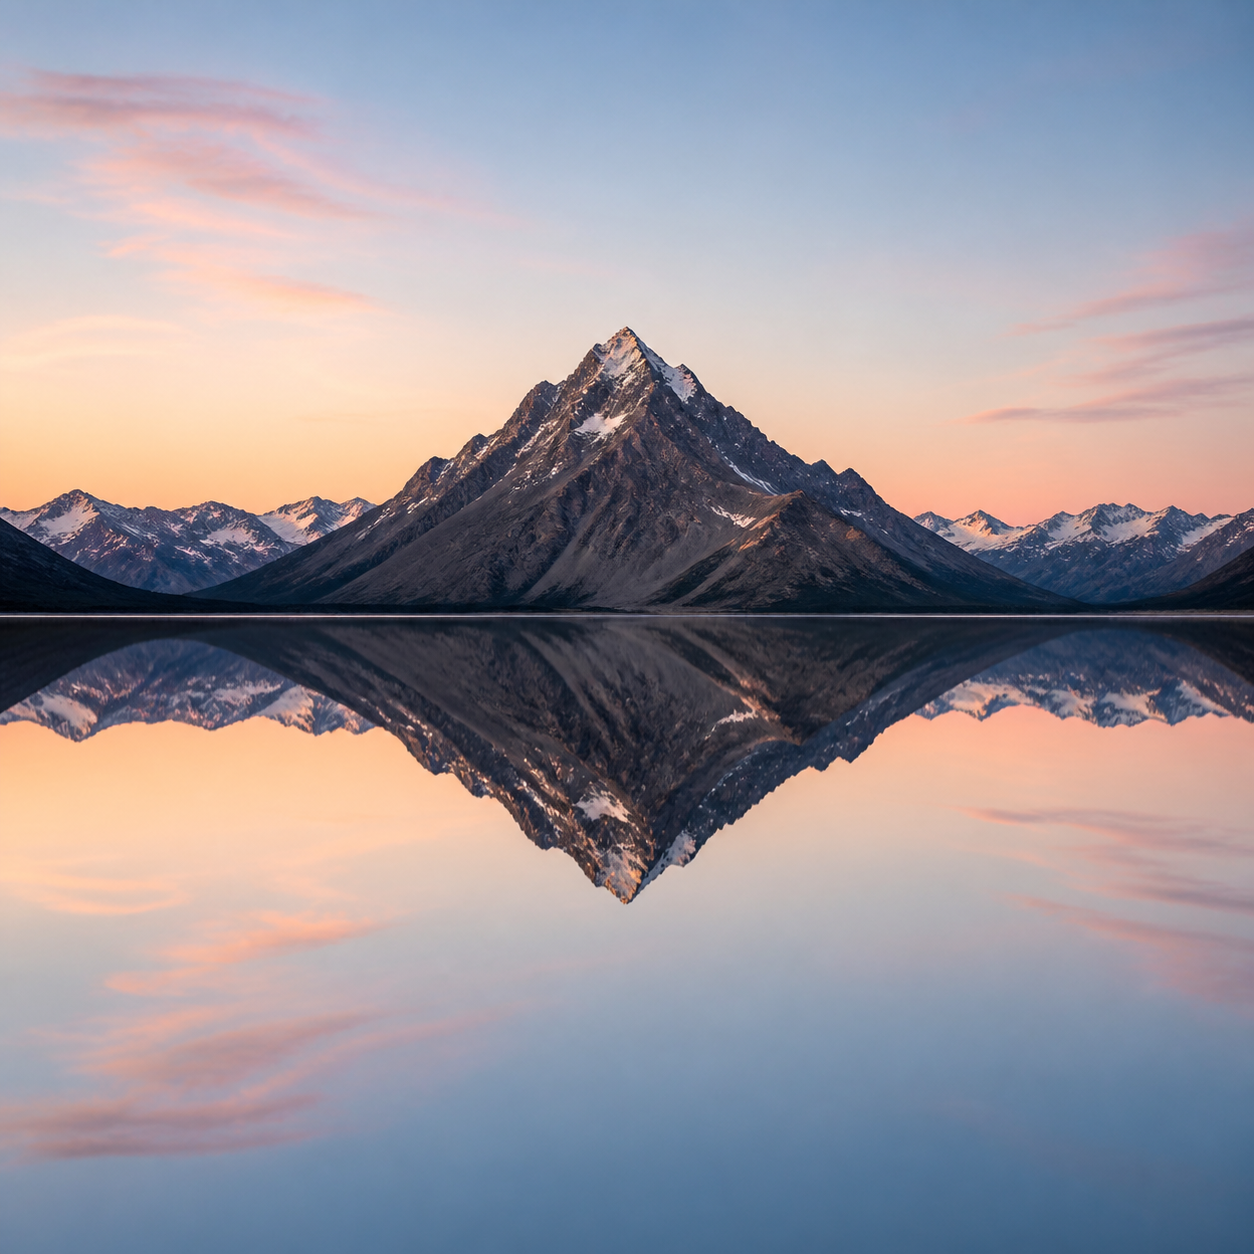
\includegraphics[width=0.45\linewidth]{images/book1/ai/g5-mirrors-lake.png}

{\small البحيرة الساكنة \omterm{def:g5:mirrors-reflection:reflection}{مرآة} مستلقية: كل شعاع يرتدّ بالقاعدة نفسها، فيظهر الجبل من جديد، مقلوبًا ودقيقًا.}
\end{omfigure}

\section{الشخص الذي خلف الزجاج}

\begin{proposition}[قاعدة الصورة]\label{prop:g5:mirrors-reflection:image}
تُظهر \omterm{def:g5:mirrors-reflection:reflection}{المرآة} المستوية كل جسم \emph{صورةً}\index{صورة} قائمة
\emph{خلف} الزجاج، على البعد نفسه الذي يقف به الجسم أمامه،
مطابقة له في الحجم، نقطةً بنقطة. تراجع فتتراجع صورتك معك؛ فعالم
\omterm{def:g5:mirrors-reflection:reflection}{المرآة} نسخة أمينة مطويّة من عالمنا.
\end{proposition}

\begin{omfigure}
\begin{tikzpicture}[scale=0.85]
  \draw[very thick] (5.5,0) -- (5.5,3.6);
  \fill[omThm] (2.5,2.6) circle (0.16);
  \draw[thick] (2.5,0.8) -- (2.5,2.4);
  \node[below, font=\small] at (2.5,0.5) {شمعة، \qty{1}{m} أمام};
  \fill[omThm, opacity=0.35] (8.5,2.6) circle (0.16);
  \draw[thick, omExo, dashed] (8.5,0.8) -- (8.5,2.4);
  \node[below, font=\small] at (8.5,0.5) {صورة، \qty{1}{m} خلف};
  \draw[omThm, thick] (2.5,2.6) -- (5.5,1.9);
  \draw[-Stealth, omThm, thick] (5.5,1.9) -- (3.4,0.35);
  \draw[omExo, dashed] (5.5,1.9) -- (8.5,2.6);
  \node[font=\small] at (3.2,0.15) {عين};
\end{tikzpicture}

{\small قاعدة الصورة: تستقبل العين شعاعًا مرتدًّا، لكنها تمدّه
مستقيمًا إلى الوراء --- إلى شمعة تبدو قائمة خلف الزجاج، على
البعد الذي تقف به الشمعة الحقيقية أمامه.}
\end{omfigure}

\begin{example}[لماذا تسكن الصورة خلف الزجاج]\label{ex:g5:mirrors-reflection:why}
عينك بسيطة الطبع: تفترض أن كل شعاع سافر مستقيمًا. والشعاع
المرتدّ يأتي حقًّا من الشمعة عبر \omterm{def:g5:mirrors-reflection:reflection}{المرآة} --- لكن العين تمدّه
\emph{إلى الوراء عبر الزجاج}، إلى الموضع الذي يبدو أنه بدأ منه.
وكل الأشعّة المرتدّة تتّفق على نقطة البدء الوهمية تلك: أشعّة
شمعة واحدة، وشمعة وهمية واحدة حادّة. ولا شيء خلف الجدار طبعًا
--- فالصورة أشدّ أوهام \omterm{def:g1:light-and-shadows:source}{الضوء} إقناعًا.
\end{example}

\begin{example}[العالَم المقلوب]\label{ex:g5:mirrors-reflection:swap}
قرّب صفحة مكتوبة من \omterm{def:g5:mirrors-reflection:reflection}{المرآة}: ترجع الحروف مقلوبة، وقد تبادل اليمين
واليسار موضعيهما. ولهذا تُكتب كلمة إسعاف مقلوبة في \omterm{def:g5:mirrors-reflection:reflection}{المرآة} على
مقدّمة سيارات الإسعاف: فالسائقون أمامها، حين يلمحونها في مرايا
الرؤية الخلفية، يرونها ترتدّ إلى قراءة سليمة --- فيفسحون الطريق.
ومرآتان تستطيعان أن تنقضا القلب: فارتداد مزدوج يقلب القلب.
\end{example}

\section{طيّ الطريق عن قصد}

\begin{method}[كيف تبني منظارًا مزواةً]\label{met:g5:mirrors-reflection:periscope}
ناظرُ الزوايا الموعود، وقد سُلّم:
\begin{enumerate}
  \item خذ علبة طويلة ضيّقة؛ واقطع نافذة قرب أعلى أحد وجهيها
        وأخرى قرب أسفل الوجه المقابل؛
  \item وثبّت \omterm{def:g5:mirrors-reflection:reflection}{مرآة} صغيرة في الداخل خلف كل نافذة، كل واحدة مائلة
        بنصف زاوية قائمة، والميلان متوازيان؛
  \item وصوّب النافذة العليا فوق الجدار (أو حول الزاوية)، وانظر
        في النافذة السفلى.
\end{enumerate}
فينطوي طريق \omterm{def:g1:light-and-shadows:source}{الضوء} مرتين: نزولًا في العلبة بين المرآتين، ثم
خروجًا إلى عينك. وأطقم الغوّاصات تراقب الأمواج بهذا بعينه ---
مبنيًّا طويلًا محكم الغلق.
\end{method}

\begin{omfigure}
\begin{tikzpicture}[scale=0.85]
  \draw[thick] (4.0,0) rectangle (5.6,4.4);
  \draw[very thick, omDef] (4.15,3.4) -- (5.45,4.25);
  \draw[very thick, omDef] (4.15,0.15) -- (5.45,1.0);
  \draw[-Stealth, omThm, very thick] (1.0,3.83) -- (4.8,3.83);
  \draw[-Stealth, omThm, very thick] (4.8,3.83) -- (4.8,0.58);
  \draw[-Stealth, omThm, very thick] (4.8,0.58) -- (8.4,0.58);
  \node[left, font=\small] at (0.9,3.83) {ضوء من المشهد};
  \node[right, font=\small] at (8.5,0.58) {إلى عينك};
  \node[right, font=\small, omDef] at (5.7,4.0) {مرآة مائلة};
  \node[right, font=\small, omDef] at (5.7,1.2) {مرآة مائلة};
\end{tikzpicture}

{\small داخل المنظار المزواة: مرآتان مائلتان متوازيتان تطويان
طريق \omterm{def:g1:light-and-shadows:source}{الضوء} مرتين --- فوق الجدار ثم إلى عينك.}
\end{omfigure}

\begin{remark}[ملاعق مدينة الملاهي]\label{rem:g5:mirrors-reflection:curved}
انظر في تجويف ملعقة مصقولة: تجد نفسك معلّقًا مقلوبًا. واقلبها:
تعود معتدلًا، لكنك ممطوط. والمرايا المنحنية تظلّ تطيع قاعدة
الارتداد عند كل نقطة --- لكن ميولها تدور مع الانحناء، فتتجمّع
الارتدادات المنظَّمة أو تتبدّد، فتصغر الصور أو تكبر أو تنقلب.
والمرايا المنحنية تجمّع \omterm{def:g1:light-and-shadows:source}{الضوء} أيضًا: فطبق منحنٍ من \omterm{def:g1:light-and-shadows:source}{ضوء} الشمس
يستطيع أن يطبخ قِدرًا --- وتذكّر الطبّاخات الشمسية في فصل
\omterm{def:g5:everyday-energy:energy}{الطاقة}. وقوانينها الدقيقة تخصّ سنة لاحقة؛ والملعقة عرضها الأمين
المسبق.
\end{remark}

\section{تمارين}

\begin{exercise}[$\star$]\label{exo:g5:mirrors-reflection:1}
اذكر قاعدة الارتداد. وماذا يفعل شعاع يصل عموديًّا؟
\end{exercise}

\begin{exercise}[$\star$]\label{exo:g5:mirrors-reflection:2}
الجدار الأبيض يعكس ضوءًا كثيرًا. فلماذا لا يُظهر صورة بينما
تُظهرها \omterm{def:g5:mirrors-reflection:reflection}{المرآة} المصقولة؟
\end{exercise}

\begin{exercise}[$\star$]\label{exo:g5:mirrors-reflection:3}
تقف على بعد \qty{2}{m} أمام \omterm{def:g5:mirrors-reflection:reflection}{مرآة} مستوية. فأين صورتك، وكم تبعد
عنك؟
\end{exercise}

\begin{exercise}[$\star$]\label{exo:g5:mirrors-reflection:4}
تمشي نحو صورتك في \omterm{def:g5:mirrors-reflection:reflection}{المرآة} بخطوة بطيئة. فماذا تفعل الصورة، وبأيّ
سرعة تنغلق المسافة بينكما؟
\end{exercise}

\begin{exercise}[$\star$]\label{exo:g5:mirrors-reflection:5}
لماذا تُكتب كلمة إسعاف مقلوبة على مقدّمة سيارات الإسعاف؟ ولمن
تُقرأ صحيحة، وعبر ماذا؟
\end{exercise}

\begin{exercise}[$\star$]\label{exo:g5:mirrors-reflection:6}
في المنظار المزواة، كم مرة ينطوي طريق \omterm{def:g1:light-and-shadows:source}{الضوء}، وماذا تطوي كل
طيّة؟ وبأيّ ميل تقف المرآتان؟
\end{exercise}

\begin{exercise}[$\star$]\label{exo:g5:mirrors-reflection:7}
كيف يستطيع متنزّه معه \omterm{def:g5:mirrors-reflection:reflection}{مرآة} جيب أن يشير إلى مروحية بعيدة؟ وأيّ
فكرتين من الفصل تعملان --- سمِّ القاعدة التي تصوّب الومضة
والمخزن الذي يشغّلها.
\end{exercise}

\begin{exercise}[$\star$]\label{exo:g5:mirrors-reflection:8}
الماء الساكن يعكس الجبال؛ وتُموّج \omterm{def:g2:air-around-us:wind}{الريح} البحيرة فتتحطّم الصورة
بريقًا متناثرًا. اشرح الحالتين بما في
\cref{ex:g5:mirrors-reflection:walls}.
\end{exercise}

\begin{exercise}[$\star\star$]\label{exo:g5:mirrors-reflection:9}
العين ``تمدّ الأشعّة إلى الوراء''. استعمل هذا لتشرح لماذا تقف
صورتك \emph{خلف} الجدار المعلّقة عليه \omterm{def:g5:mirrors-reflection:reflection}{المرآة} --- في موضع لا يقف
فيه أحد قطعًا. وعلى أيّ شيء تتّفق كل الأشعّة المرتدّة عن أنفك؟
\end{exercise}

\begin{exercise}[$\star\star$]\label{exo:g5:mirrors-reflection:10}
يريد متجر أن يرى زبون عند الباب ما وراء زاوية عمياء في الممرّ.
ويجب أن تُركَّب \omterm{def:g5:mirrors-reflection:reflection}{مرآة} مستوية واحدة حيث يلتقي الممرّان. فكيف
ينبغي أن تُمال، ولماذا يتيح التركيب نفسه للممرّ أن يرى الباب؟
(فطرق \omterm{def:g1:light-and-shadows:source}{الضوء} تعمل في الاتجاهين.)
\end{exercise}

\begin{exercise}[$\star\star$]\label{exo:g5:mirrors-reflection:11}
الكتابة في \omterm{def:g5:mirrors-reflection:reflection}{المرآة} ترجع مقلوبة؛ والارتداد المزدوج ``يقلب
القلب''. اشرح لماذا يُظهر المنظار المزواة في
\cref{met:g5:mirrors-reflection:periscope}، بمرآتيه، المشهدَ
معتدلًا لا مقلوبًا في \omterm{def:g5:mirrors-reflection:reflection}{المرآة}.
\end{exercise}
